%----------------------------------------------------------------------------------------
%   SIMULACIONES
%----------------------------------------------------------------------------------------

\chapter{Simulaciones}

\label{ch:simulaciones}

Debido a las limitaciones de tiempo y recursos para realizar el trabajo de
investigación, la evaluación del protocolo propuesto se llevó a cabo mediante
simulaciones. Se utilizó la herramienta SUMO, que permite crear modelos de las
redes viales y hacer la simulación del movimiento de los vehículos \cite{SUMO}.
Para simular la comunicación entre los vehículos, se utilizó OMNeT++, un
simulador de eventos discretos muy usado para evaluar protocolos de
comunicación \cite{OMNeT}, además del \textit{framework} INET, que incluye
modelos de muchos protocolos estándar, como la pila de protocolos TCP/IP
\cite{INET}. Para simular la red de vehículos, se utilizó el \textit{framework}
Veins, que permite la interacción entre la simulación de vehículos de SUMO y la
simulación de comunicaciones de OMNeT++ \cite{Veins}. Por otro lado, se utilizó
el programa JOSM para descargar y acondicionar mapas de OpenStreetMap, que se
utilizan para crear la simulación de los vehículos \cite{OpenStreetMap}
\cite{JOSM}, y se utilizó QGIS para crear los grafos viales de las subredes
\cite{QGIS}.

En este capítulo, se explica cómo se utilizaron estas herramientas para el
desarrollo de las simulaciones que se llevaron a cabo para evaluar el desempeño
del protocolo propuesto.

%----------------------------------------------------------------------------------------
%	INSTALACIÓN DE LAS HERRAMIENTAS
%----------------------------------------------------------------------------------------

\section{Instalación de las herramientas}

\label{sec:instalacion_herramientas}

A continuación, se explica cómo instalar las herramientas utilizadas para
realizar las simulaciones en el sistema operativo Fedora 33, que se utilizó
para el desarrollo.

%----------------------------------------------------------------------------------------
%   INSTALACIÓN DE SUMO
%----------------------------------------------------------------------------------------

\subsection{Instalación de SUMO}

\label{subsec:instalacion_sumo}

Primero, se descarga el
\href{https://sourceforge.net/projects/sumo/files/sumo/}{código fuente de SUMO
1.8.0}, y se descomprime el directorio {\lstinline[language=bash]!sumo-1.8.0!}
dentro del directorio {\lstinline[language=bash]!~/src!}. Después, se instalan
los paquetes requeridos con los siguientes comandos:

\begin{lstlisting}[language=bash]
$ sudo dnf install cmake python gcc-c++ xerces-c-devel fox-devel \
    gdal-devel proj-devel gl2ps-devel OpenSceneGraph-devel python3-devel \
    swig gtest-devel eigen3-devel python3-pip java-11-openjdk-devel \
    mesa-libGLU-devel libXext-devel fontconfig-devel libXft-devel \
    libXcursor-devel libXrender-devel libXrandr-devel libXfixes-devel \
    libXi-devel libjpeg-turbo-devel libtiff-devel
$ pip3 install texttest
$ sudo dnf -y install https://download1.rpmfusion.org/free/fedora/\
    rpmfusion-free-release-$(rpm -E %fedora).noarch.rpm
$ sudo dnf -y install https://download1.rpmfusion.org/nonfree/fedora/\
    rpmfusion-nonfree-release-$(rpm -E %fedora).noarch.rpm
$ sudo dnf install ffmpeg-devel
\end{lstlisting}

Para compilar el código fuente, se ejecutan los siguientes comandos:

\begin{lstlisting}[language=bash]
$ cd $HOME/src/sumo-1.8.0
$ export SUMO_HOME=$HOME/src/sumo-1.8.0
$ mkdir build/cmake-build
$ cd build/cmake-build
$ cmake ../..
$ make -j $(nproc)
\end{lstlisting}

Para que SUMO esté disponible en la variable de entorno permanentemente
{\lstinline[language=bash]!PATH!}, se agregan las siguientes líneas al archivo
{\lstinline[language=bash]!~/.bashrc!}:

\begin{lstlisting}[language=bash]
export SUMO_HOME=$HOME/src/sumo-1.8.0
export PATH=$SUMO_HOME/bin:$PATH
export PATH=$SUMO_HOME/tools:$PATH
\end{lstlisting}

Las instrucciones de compilación detalladas se pueden consultar en
\cite{CompilacionSUMO}.

Evaluación de protocolos de enrutamiento: \cite{Nishat2011}.

%-----------------------------------
%	INSTALACIÓN DE OMNET++
%-----------------------------------
\subsection{Instalación de OMNeT++}

\label{subsec:instalacion_omnet}

Primero, se descarga el \href{https://omnetpp.org/download/}{código fuente de
OMNeT++ 5.6.2}, y se descomprime el directorio
{\lstinline[language=bash]!omnetpp-5.6.2!} dentro del disrectorio
{\lstinline[language=bash]!~/src!}. Después, se instalan los paquetes
requeridos con el siguiente comando:

\begin{lstlisting}[language=bash]
$ sudo dnf install make gcc gcc-c++ bison flex perl python2 tcl-devel \
    tk-devel qt5-qtbase-devel libxml2-devel zlib-devel doxygen graphviz \
    webkit2gtk3-devel OpenSceneGraph-devel osgearth-devel openmpi-devel
\end{lstlisting}

Para compilar el código fuente, se ejecutan los siguientes comandos:

\begin{lstlisting}[language=bash]
$ cd $HOME/src/omnetpp-5.6.2
$ . setenv
$ ./configure
$ make
\end{lstlisting}

Para que OMNeT++ esté disponible en la variable de entorno
{\lstinline[language=bash]!PATH!}, se agrega la siguiente línea al archivo
{\lstinline[language=bash]!~/.bashrc!}:

\begin{lstlisting}[language=bash]
export PATH=$HOME/src/omnetpp-5.6.2:$PATH
\end{lstlisting}

Las instrucciones de compilación detalladas se pueden consultar en
\cite{CompilacionOMNeT}.

%-----------------------------------
%   INSTALACIÓN DE QGIS
%-----------------------------------

\subsection{Instalación de QGIS}

\label{subsec:instalacion_qgis}

Para instalar QGIS 3.16, se ejecutan los siguientes comandos:

\begin{lstlisting}[language=bash]
$ sudo dnf copr enable dani/qgis
$ sudo dnf install qgis python3-qgis qgis-grass
\end{lstlisting}

Se pueden consultar más detalles sobre la instalación en
\cite{InstalacionQGIS}.

%----------------------------------------------------------------------------------------
%	INSTALACIÓN DE JOSM
%----------------------------------------------------------------------------------------

\subsection{Instalación de JOSM}

\label{subsec:instalacion_josm}

JOSM es una aplicación Java, por lo que primero se debe instalar la máquina
virtual de Java con el siguiente comando:

\begin{lstlisting}[language=bash]
$ sudo dnf install java-11-openjdk
\end{lstlisting}

Después, se descarga el
\href{https://josm.openstreetmap.de/wiki/Download}{archivo
\code{josm-tested.jar}}, y la aplicación se ejecuta con el siguiente comando:

\begin{lstlisting}[language=bash]
$ java -jar josm-tested.jar
\end{lstlisting}

Se pueden consultar más detalles en \cite{DescargaJOSM}.

%----------------------------------------------------------------------------------------
%   CREACIÓN DE LA BASE DE DATOS DE GRAFOS VIALES
%----------------------------------------------------------------------------------------

\section{Creación de la base de datos de grafos viales}

\label{sec:creacion_base_de_datos_de_grafos_viales}

\begin{sloppypar}
Los vehículos deben conocer la topología de la red vial de la subred donde se
encuentran, por lo que tienen que contar con una base de datos que contenga los
grafos viales de las subredes. Para crear cada grafo vial, se utilizó como
referencia una capa de OpenStreetMap en QGIS. Se creó una capa vectorial de
puntos, en la que se colocó un punto en cada cruce vial, que representan los
vértices del grafo. Después, se creó una capa vectorial de líneas, en la que se
creó una línea para cada segmento de calles, que representan las aristas del
grafo. La capa de vértices se guardó en un archivo Shapefile llamado
\code{vertices.shp}, y la capa de aristas en un archivo llamado
\code{aristas.shp}. En el archivo \code{vertices.shp}, cada registro tiene el
campo \code{GATEWAY} de tipo entero, cuyo valor tiene el siguiente significado:
\end{sloppypar}

\begin{tabular}{ r l }
0 & No es \textit{gateway} \\
1 & \textit{Gateway} norte \\
2 & \textit{Gateway} este \\
3 & \textit{Gateway} sur \\
4 & \textit{Gateway} oeste \\
\end{tabular}

En la figura \ref{fig:qgis_grafo_vial}, se muestra cómo se crearon los
archivos Shapefile en QGIS de la subred 9g3qxs. Los puntos que representan los
vértices se muestran como círculos cuyo color representa el tipo de
\textit{gateway} que es. Las aristas se muestran como líneas de color azul.

\begin{figure}[th!]
\centering
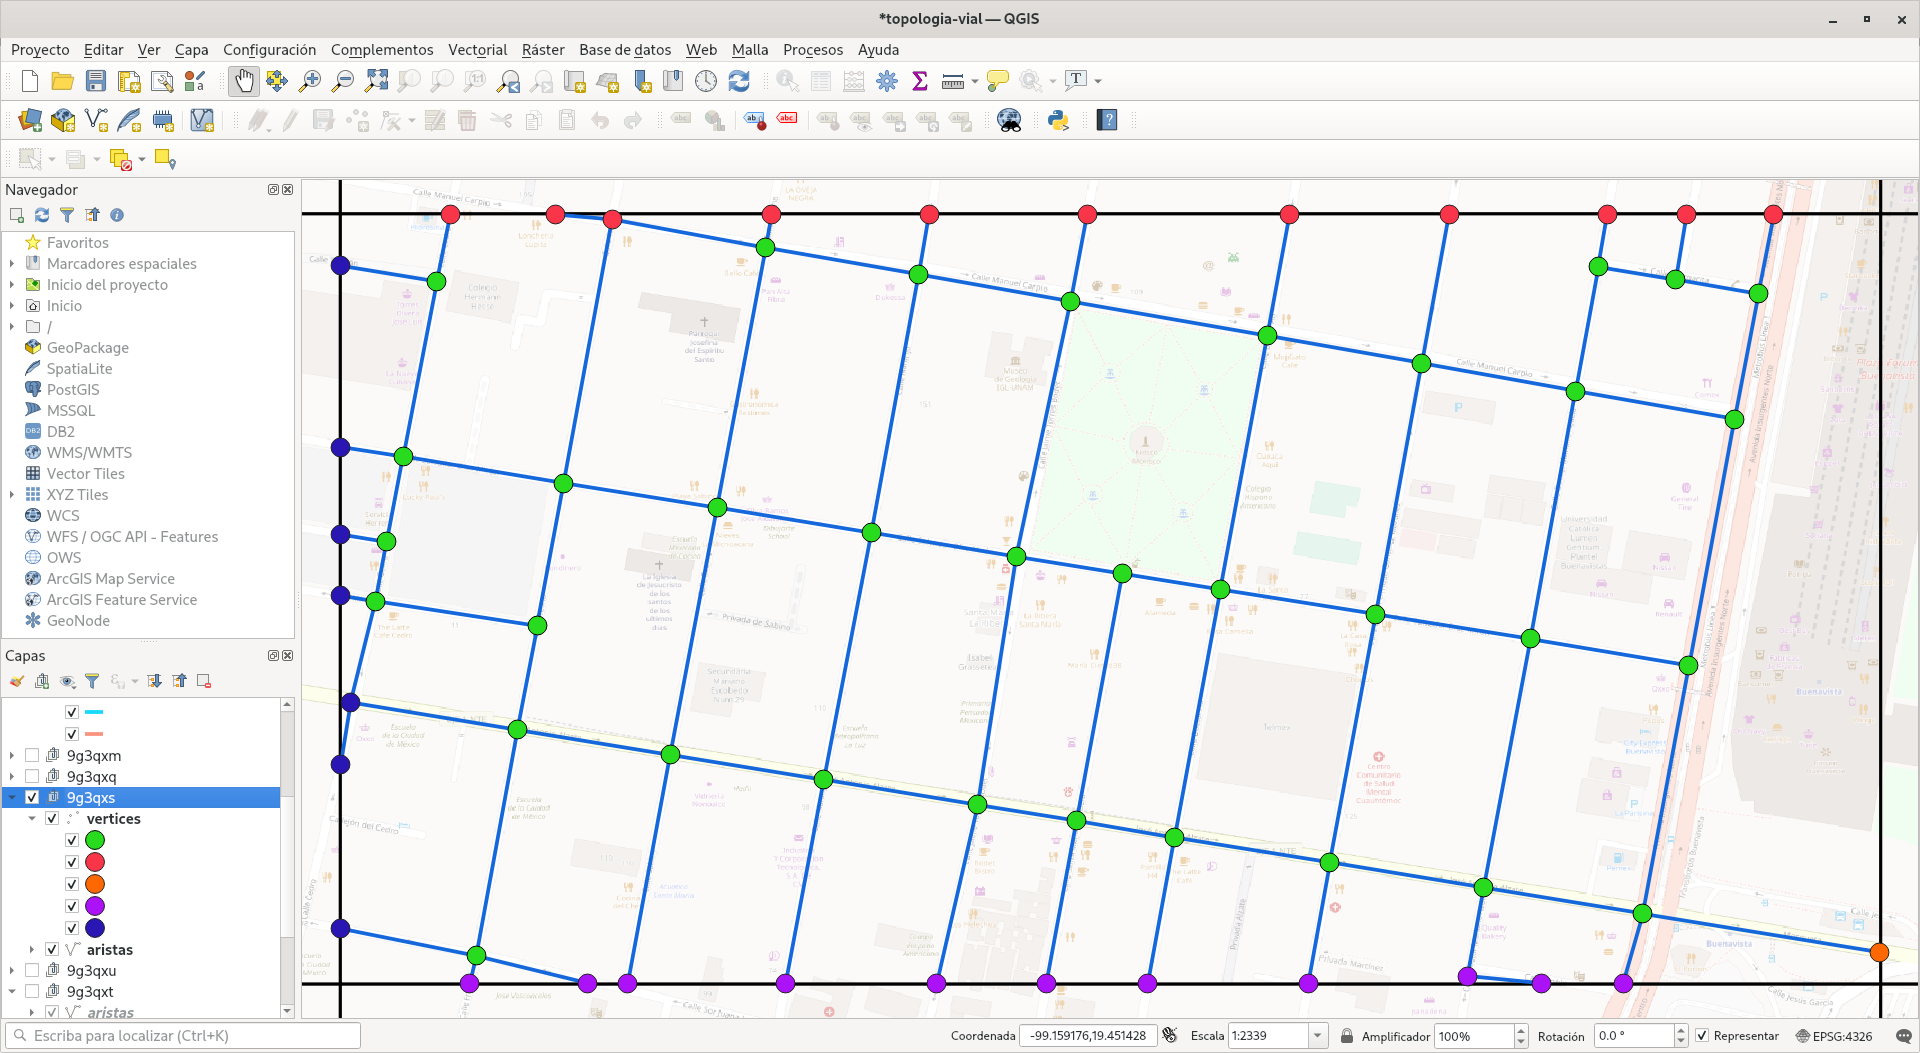
\includegraphics[width=1\textwidth]{qgis_grafo_vial}
\decoRule
\caption[Grafo vial en QGIS]{Grafo vial en QGIS.}
\label{fig:qgis_grafo_vial}
\end{figure}

Por conveniencia, se utilizaron los archivos \code{vertices.shp} y
\code{aristas.shp} para crear un archivo XML llamado \code{grafo-vial-\{subred
geohash\}.xml} que contiene la misma información, pero con otro formato. Este
contiene un nodo \code{grafo-vial}, que contiene dos nodos: \code{vertices} y
\code{aristas}. El nodo \code{vertices} contiene una lista de nodos
\code{vertice}, y cada uno contiene información sobre su ubicación y el tipo de
\textit{gateway} del vértice en sus atributos. El nodo \code{aristas} contiene
una lista de nodos \code{arista}, que especifican el par de vértices que forma
cada arista. Por ejemplo, el archivo \code{grafo-vial-9g3qxs.xml} es el
siguiente:

\begin{lstlisting}[language=XML]
<?xml version="1.0" ?>
<grafo-vial>
    <vertices>
        <vertice lat="19.446002168" lon="-99.161628593" gateway="0"/>
        <vertice lat="19.445807675" lon="-99.160834191" gateway="3"/>
        <vertice lat="19.445804060" lon="-99.160548559" gateway="3"/>
        <vertice lat="19.445804060" lon="-99.159421395" gateway="3"/>
        <vertice lat="19.445804060" lon="-99.158343042" gateway="3"/>
        ...
    </vertices>
    <aristas>
        <arista vertice1="0" vertice2="19"/>
        <arista vertice1="19" vertice2="24"/>
        <arista vertice1="24" vertice2="28"/>
        <arista vertice1="28" vertice2="44"/>
        <arista vertice1="45" vertice2="44"/>
        ...
    </aristas>
</grafo-vial>
\end{lstlisting}

Ya que se necesita que cada vehículo conozca la topología vial para cada una de
las subredes, la base de datos de grafos viales consiste en el conjunto de
archivos XML de los grafos viales de cada subred dentro del directorio
\code{bd-grafos-viales}, como se muestra a continuación:

\dirtree{%
.1 src.
    .2 bd-grafos-viales.
        .3 grafo-vial-9g3qxk.xml.
        .3 grafo-vial-9g3qxm.xml.
        .3 grafo-vial-9g3qxq.xml.
        .3 grafo-vial-9g3qxs.xml.
        .3 grafo-vial-9g3qxt.xml.
        .3 \ldots.
}

%----------------------------------------------------------------------------------------
%   SIMULACIÓNES DE SUMO
%----------------------------------------------------------------------------------------

\section{Simulaciones de SUMO}

\label{sec:simulaciones_sumo}

Para hacer una simulación del movimiento de los vehículos, primero se necesita
tener una definición de una red vial por la que los vehículos puedan circular.
Para esto, primero se utiliza JOSM para descargar desde OpenStreetMap un
archivo OSM que contiene el mapa de la región de interés. Para descargar un
mapa, hay que indicar la región que la delimita. En la figura
\ref{fig:josm_descargar_region}, se muestra cómo descargar la región Geohash
9g3qxs, que se encuentra entre la latitud 19.4458007812 y 19.4512939453, y
entre la longitud -99.1625976562 y -99.1516113281.

\begin{figure}[th!]
\centering
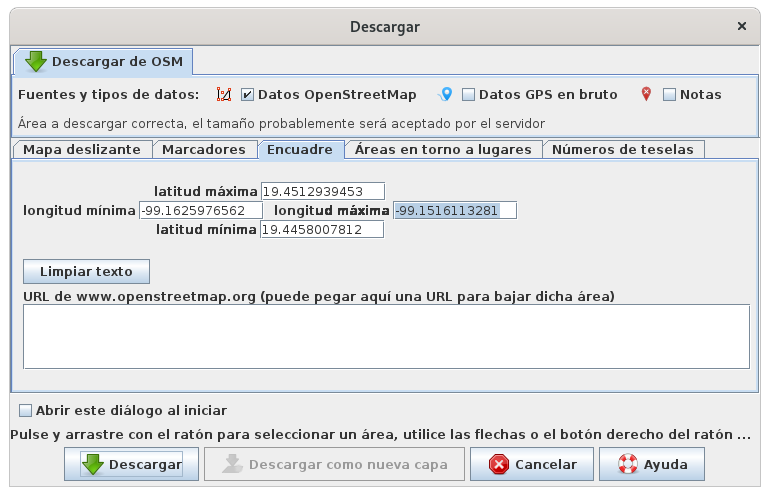
\includegraphics[width=1\textwidth]{josm_descargar_region}
\decoRule
\caption[Descargar mapa de la región Geohash 9g3qxs en JOSM]{Descargar mapa de
la región Geohash 9g3qxs en JOSM.}
\label{fig:josm_descargar_region}
\end{figure}

Por defecto, el mapa descargado incluye elementos fuera de la región de
interés, además de que muchas de las vialidades se extienden fuera de esta,
como se muestra en la figura \ref{fig:josm_mapa_descargado}. Por esta razón, se
utiliza JOSM también para eliminar los elementos que son innecesarios y
recortar los segmentos de las vialidades que se encuentran fuera de la región,
así como corregir la cantidad de carriles de las vialidades. La figura
\ref{fig:josm_mapa_acondicionado} muestra el mapa después de realizar este
procedimiento, que se guarda con el nombre \code{9g3qxs.osm}.

\begin{figure}[th!]
\centering
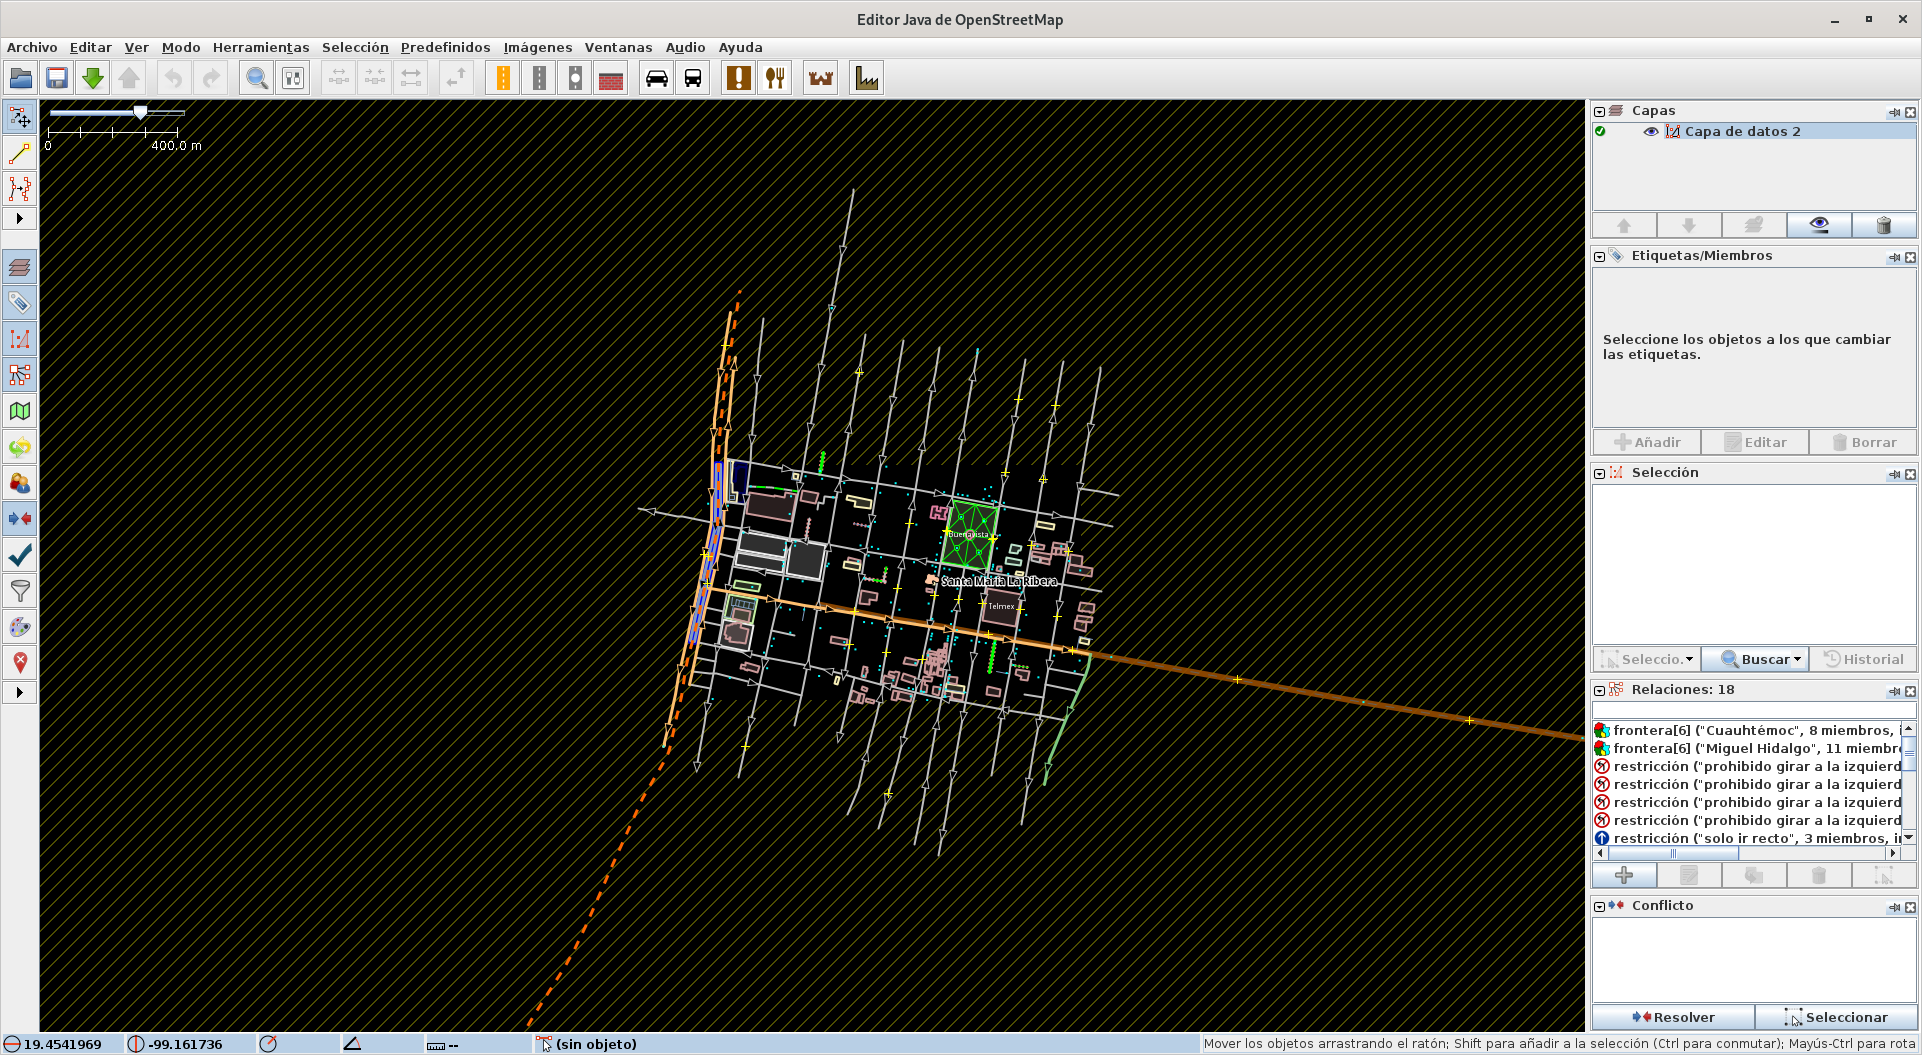
\includegraphics[width=1\textwidth]{josm_mapa_descargado} 
\decoRule
\caption[Mapa de la región Geohash 9g3qxs descargado con JOSM]{Mapa de la
región Geohash 9g3qxs descargado con JOSM.}
\label{fig:josm_mapa_descargado}
\end{figure}

\begin{figure}[th!]
\centering
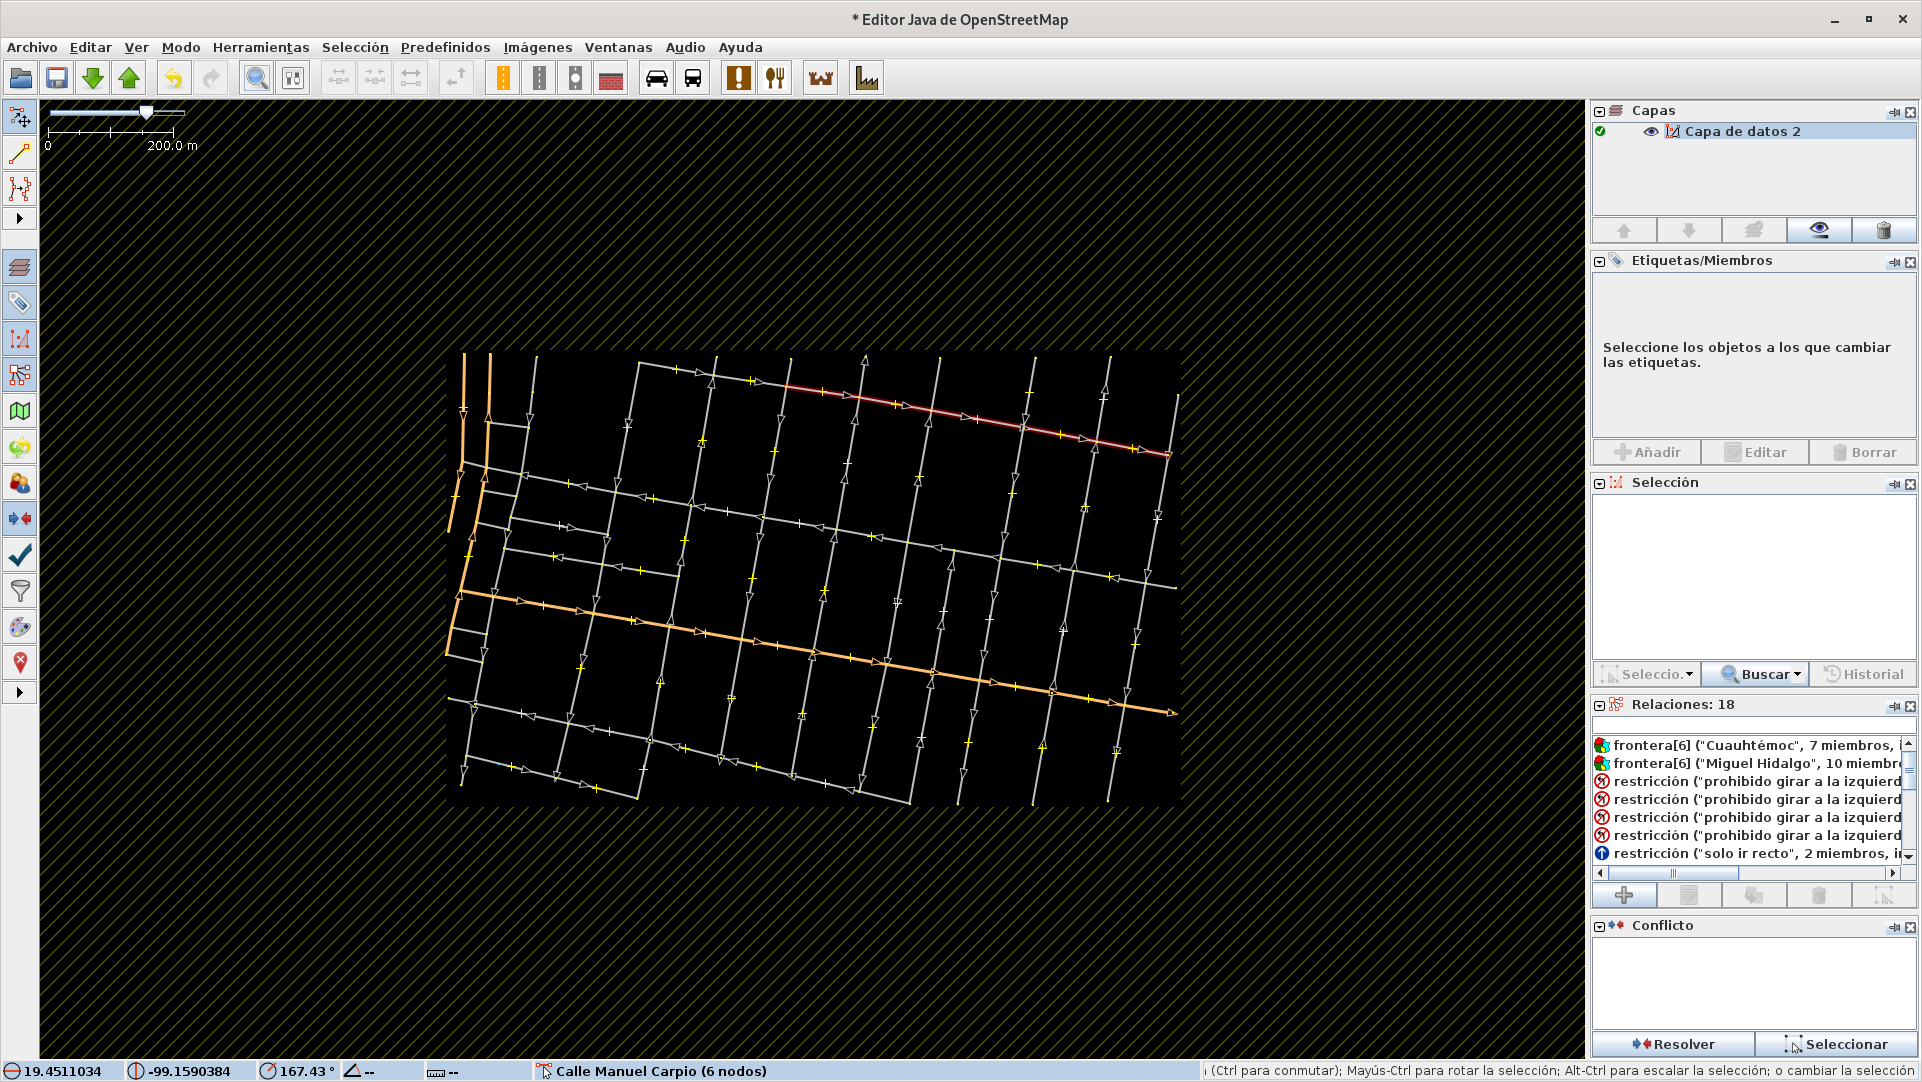
\includegraphics[width=1\textwidth]{josm_mapa_acondicionado}
\decoRule
\caption[Mapa de la región Geohash 9g3qxs acondicionado para la
simulación]{Mapa de la región Geohash 9g3qxs acondicionado para la simulación.}
\label{fig:josm_mapa_acondicionado}
\end{figure}

SUMO define su propio formato para representar las redes viales, y cuenta con
una herramienta llamada \code{netconvert}, cuyo objetivo es convertir redes
viales de diferentes formatos a redes viales de SUMO. Para obtener la red vial
\code{9g3qxs.net.xml} a partir del mapa \code{9g3qxs.osm}, se ejecuta el
siguiente comando:

\begin{lstlisting}[language=bash]
$ netconvert --osm-files 9g3qxs.osm -o 9g3qxs.net.xml
\end{lstlisting}

Se pueden consultar más detalles sobre el uso de esta herramienta con el
siguiente comando:

\begin{lstlisting}[language=bash]
$ netconvert --help
\end{lstlisting}

Una vez que se cuenta con la red vial de SUMO, se tiene que generar el tráfico
de los vehículos, que se define en otro archivo. SUMO proporciona la
herramienta \code{randomTrips.py}, que permite generar tráfico pseudoaleatorio
que se puede simular. El siguiente comando genera como salida el archivo
\code{9g3qxs.rou.xml} a partir del archivo \code{9g3qxs.net.xml}, que contiene
las rutas que van a seguir cada uno de los vehículos que serán simulados:

\begin{lstlisting}[language=bash]
$ randomTrips.py -n 9g3qxs.net.xml -r 9g3qxs.rou.xml -p 0.6 -e 60
\end{lstlisting}

La opción \code{-p} indica el intervalo de tiempo en segundos en el que
aparecerá un nuevo vehículo en la simulación, y la opción \code{-e} indica el
tiempo en segundos en el que dejarán de aparecer nuevos vehículos. Existen más
opciones que se pueden usar para obtener diferentes resultados, que se pueden
consultar con el siguiente comando:

\begin{lstlisting}[language=bash]
$ randomTrips.py --help
\end{lstlisting}

Teniendo el archivo \code{9g3qxs.net.xml} de la red vial y el archivo
\code{9g3qxs.rou.xml} del tráfico, se define el archivo \code{9g3qxs.sumocfg},
que indica la configuración de la simulación que se quiere ejecutar. El
contenido de este archivo es el siguiente:

\begin{lstlisting}[language=XML]
<?xml version="1.0" ?>
<configuration>
    <input>
        <net-file value="9g3qxs.net.xml"/>
        <route-files value="9g3qxs.rou.xml"/>
    </input>
    <time>
        <begin value="0"/>
        <end value="60"/>
        <step-length value="0.1"/>
    </time>
</configuration>
\end{lstlisting}

Con el siguiente comando se ejecuta la simulación de manera gráfica:

\begin{lstlisting}[language=bash]
$ sumo-gui -c 9g3qxs.sumocfg
\end{lstlisting}

Se pueden consultar más detalles sobre el uso de esta herramienta con el
siguiente comando:

\begin{lstlisting}[language=bash]
$ sumo-gui --help
\end{lstlisting}

Al ejecutar la simulación, se muestra la red vial y una animación del
movimiento de los vehículos en el tiempo. La ventana de la simulación se muestra
en la figura \ref{fig:sumo_simulacion}.

\begin{figure}[th!]
\centering
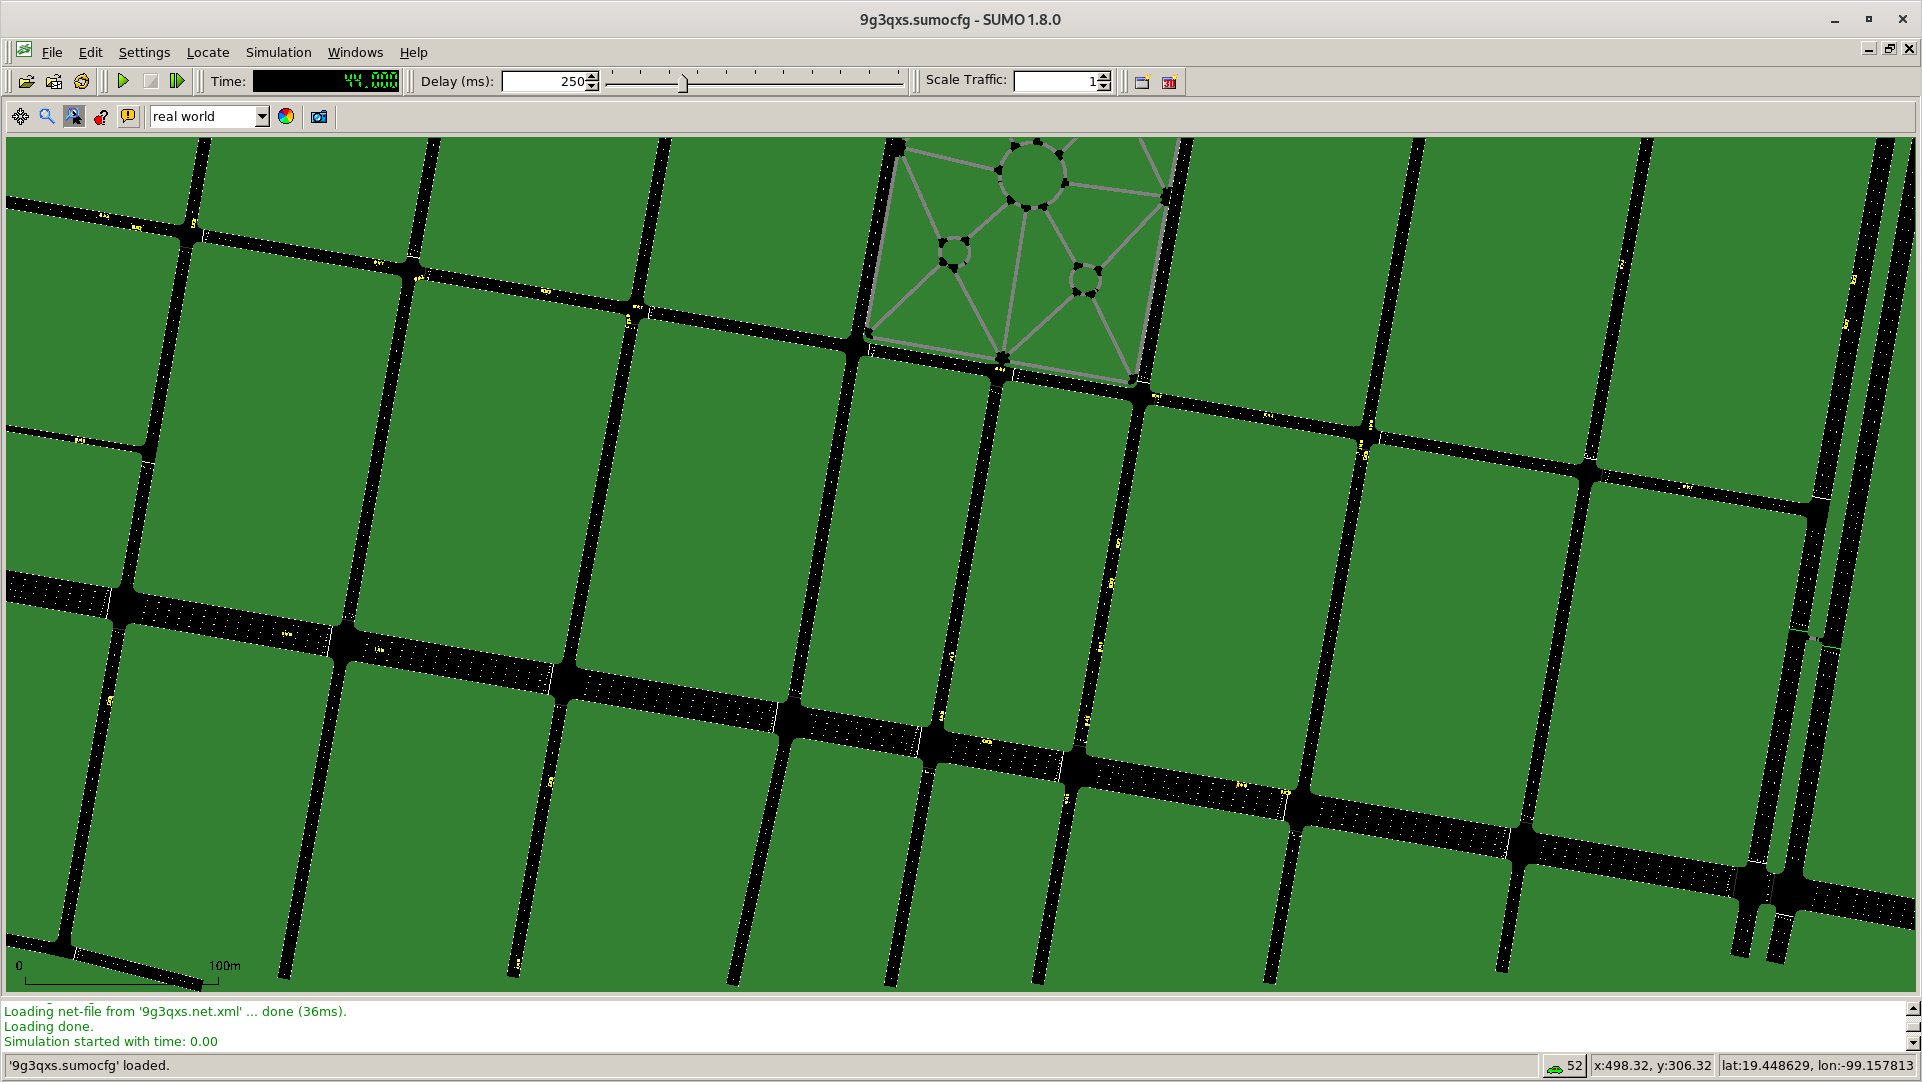
\includegraphics[width=1\textwidth]{sumo_simulacion}
\decoRule
\caption[Simulación de SUMO]{Simulación de SUMO.}
\label{fig:sumo_simulacion}
\end{figure}

%----------------------------------------------------------------------------------------
%   PROYECTO DE OMNET++
%----------------------------------------------------------------------------------------

\section{Proyecto de OMNeT++}

\label{sec:proyecto_omnet}

El proyecto de Veins es un proyecto de OMNeT++ que utiliza el
\textit{framework} Veins en conjunto con la simulación de vehículos de SUMO y
Veins para crear la simulación de la VANET. En esta sección, se muestra la
creación y el desarrollo del proyecto.

%-----------------------------------
%   CREACIÓN DEL PROYECTO
%-----------------------------------

\subsection{Creación del proyecto}

\label{subsec:creacion_proyecto}

\begin{sloppypar}
La manera recomendada de crear un proyecto de Veins es utilizar la plantilla
\code{cookiecutter-veins-project} utilizando la herramienta Cookiecutter
\cite{Cookiecutter}. Para instalar Cookiecutter, se ejecuta el siguiente
comando:
\end{sloppypar}

\begin{lstlisting}[language=bash]
$ pip3 install --user cookiecutter
\end{lstlisting}

El proyecto \code{veins\_proj} se crea dentro del directorio
{\lstinline[language=bash]!~/src!}, y se necesita utilizar el
\textit{framework} INET, por lo que la plantilla se crea y se configura de la
siguiente manera:

\begin{lstlisting}[language=bash]
$ cookiecutter -o $HOME/src/ gh:veins/cookiecutter-veins-project
project_name [Veins Proj]:
project_brief [Sample combination of Veins and a custom
project]: Protocolo de enrutamiento para VANETs
project_name_as_file_name [veins_proj]:
project_name_as_macro_name [VEINS_PROJ]:
Select use_inet: 2
1 - no
2 - yes
Choose from 1, 2 (1, 2) [1]:
Select use_inet3:
1 - no
2 - yes
Choose from 1, 2 (1, 2) [1]:
Select use_veins_vlc:
1 - no
2 - yes
Choose from 1, 2 (1, 2) [1]:
Select use_plexe_veins:
1 - no
2 - yes
Choose from 1, 2 (1, 2) [1]:
Select use_simulte:
1 - no
2 - yes
Choose from 1, 2 (1, 2) [1]:
Cookiecutter checks starting.
Making sure we can run git
git version 2.23.0
Cookiecutter checks successful.
Cookiecutter successful. Running git commands to set up
repository.
[...]
From https://github.com/sommer/veins
 * tag               veins-5.1  -> FETCH_HEAD
Added dir 'veins'
Repository set up successful. Running git commands to clean
up.
Cookiecutter successful.
\end{lstlisting}

Se puede consultar más sobre el uso de Veins en \cite{TutorialVeins}.

La plantilla incluye el proyecto \code{inet}, que es el \textit{framework} INET
que proporciona modelos de protocolos de comunicación estandarizados; el
proyecto \code{veins} es el \code{framework} Veins, que permite utilizar SUMO
para simular el movimiento de los vehículos en OMNeT++; y el proyecto
\code{veins\_inet}, que permite utilizar los modelos proporcionados por INET en
conjunto con SUMO. El proyecto \code{veins\_proj} es el proyecto en el que se
programa el funcionamiento del protocolo propuesto, y depende de los demás
proyecto. Después de importar los proyectos al espacio de trabajo de OMNeT++,
se tiene la siguiente estructura de directorios:

\dirtree{%
.1 src.
    .2 workspace.
        .3 inet.
        .3 veins.
            .4 \ldots.
            .4 subprojects.
                .5 \ldots.
                .5 veins\_inet.
        .3 veins\_proj.
}

%-----------------------------------
%   DESARROLLO DEL PROYECTO
%-----------------------------------

\subsection{Desarrollo del proyecto}

\label{subsec:desarrollo_proyecto}

Los proyectos en OMNeT++ se componen de módulos simples y compuestos, que son
las entidades que interactúan entre sí a lo largo del tiempo de simulación. Los
módulos se definen en un lenguaje llamado NED, que permite especificar
parámetros para definir el comportamiento de los módulos, y compuertas mediante
las cuales se comunican con otros módulos. Los \keyword{módulos simples} se
definen con un archivo NED, y una clase de C++, donde se describe su
comportamiento. Los \keyword{módulos compuestos} se definen únicamente por un
archivo NED, donde se indica los módulos simples que lo componen y cómo se
comunican entre sí.

A continuación, se explica la estructura del proyecto y cuáles son los aspectos
más importantes. Por conveniencia, se utilizó una nomenclatura similar a la que
se utiliza en INET y Veins. El código fuente se puede consultar en el siguiente
repositorio:

\begin{center}
\href{https://bitbucket.org/comecacahuates/sim/src/main/}{https://bitbucket.org/comecacahuates/sim/src/main/}
\end{center}

%-----------------------------------
%   BASE DE DATOS DE REDES VIALES
%-----------------------------------

\subsubsection{Base de datos de redes viales}

\label{subsubsec:base_de_datos_de_redes_viales}

Como se ha mencionado anteriormente, cada vehículo debe contar con una base de
datos de redes viales. Sin embargo, para optimizar los recursos de la
computadora, principalmente la memoria, en la simulación únicamente hay una
base de datos global a la que todos los vehículos tienen acceso. En el proyecto
\code{veins\_proj}, los archivos del proyecto relacionados con la base de datos
de redes viales son los siguientes:
\newpage

\dirtree{%
.1 veins\_proj.
    .2 \ldots.
    .2 src.
        .3 \ldots.
        .3 veins\_proj.
            .4 \ldots.
            .4 roadnetwork.
                .5 RoadNetworkGraph.h.
                .5 RoadNetworkGraph.cc.
                .5 RoadNetwork.h.
                .5 RoadNetwork.cc.
                .5 RoadNetworkDatabase.ned.
                .5 RoadNetworkDatabase.h.
                .5 RoadNetworkDatabase.cc.
}

En \code{RoadNetworkGraph.h}, se declaran los tipos de datos para la creación
de los grafos viales, además de algunas operaciones útiles relacionadas con
estos. Para la implementación de los grafos, se utilizó la biblioteca Boost
\cite{Boost}.

En \code{RoadNetwork.h}, define la clase \code{RoadNetwork}, que se encarga de
crear un grafo a partir de un archivo XML de la base de datos de grafos viales.
Además incluye métodos para calcular la ubicación vial de los vehículos,
calcular el peso de una arista y calcular la ruta más corta.

En \code{RoadNetworkDatabase.ned}, se define el módulo que proporciona a los
vehículos el acceso a la base de datos. Este módulo se encarga, al iniciar la
simulación, de leer los archivos XML de la base de datos de grafos viales, y
crea un objeto de la clase \code{RoadNetwork} por cada uno. Estos objetos se
almacenan en un vector durante toda la simulación, y cada vehículo es capaz de
consultar la red vial que necesite.

%-----------------------------------
%   MOVIMIENTO DE LOS NODOS
%-----------------------------------

\subsubsection{Movimiento de los nodos}

\label{subsubsec:movimiento_de_los_nodos}

En INET, el movimiento de los nodos se modela con un módulo que herede del
módulo \code{MobilityBase}. INET proporciona varios módulos que modelan
diferentes tipos de movimientos, sin embargo, Veins proporciona el módulo
\code{VeinsInetMobility}, que interactúa con SUMO para obtener la información
sobre el movimiento de los vehículos. Los archivos del proyecto relacionados
con el movimiento de los nodos de la red son los siguientes:
\newpage

\dirtree{%
.1 veins\_proj.
    .2 \ldots.
    .2 src.
        .3 \ldots.
        .3 veins\_proj.
            .4 \ldots.
            .4 mobility.
                .5 StaticHostMobility.ned.
                .5 StaticHostMobility.h.
                .5 StaticHostMobility.cc.
                .5 CarMobility.ned.
                .5 CarMobility.h.
                .5 CarMobility.cc.
}

\begin{sloppypar}
En la simulación, los \textit{hosts} se mantienen en la misma posición todo el
tiempo. El módulo \code{StaticHostMobility} permite obtener la ubicación de
cada \textit{host} en la simulación, y hereda del módulo
\code{MovingMobilityBase}, que es proporcionado por INET.
\end{sloppypar}

Para modelar el movimiento de los vehículos, se definió el módulo
\code{CarMobility}. Este módulo hereda del módulo \code{VeinsInetMobility}, e
implementa métodos para obtener la red vial de la subred donde se encuentra el
vehículo, calcular su ubicación vial, determinar si se encuentra en una arista
\textit{gateway} o si cambió de subred, y otras operaciones útiles.

%-----------------------------------
%   AUTOCONFIGURACIÓN DE DIRECCIONES
%-----------------------------------

\subsubsection{Autoconfiguración de direcciones}

\label{subsubsec:autoconfiguracion_de_direcciones_sim}

Una vez teniendo los módulos que permiten conocer la ubicación de los
dispositivos, se puede implementar la autoconfiguración de direcciones. Los
archivos en el proyecto relacionados con la autoconfiguración de direcciones
son los siguientes:

\dirtree{%
.1 veins\_proj.
    .2 \ldots.
    .2 src.
        .3 \ldots.
        .3 veins\_proj.
            .4 \ldots.
            .4 networklayer.
                .5 ipv6.
                    .6 Ipv6GeohashAddress.h.
                    .6 Ipv6GeohashAddress.cc.
                .5 configurator.
                    .6 StaticHostConfigurator.ned.
                    .6 StaticHostConfigurator.h.
                    .6 StaticHostConfigurator.cc.
                    .6 CarConfigurator.ned.
                    .6 CarConfigurator.h.
                    .6 CarConfigurator.cc.
}

En \code{Ipv6GeohashAddress.h} se incluyen funciones que generan direcciones
IPv6 \textit{unicast} y \textit{multicast} a partir de una ubicación Geohash y
el identificador EUI-64 de la interfaz.

El módulo \code{StaticHostConfigurator} obtiene la ubicación de un
\textit{host} con el módulo \code{StaticHostMobility} al inicio de la
simulación. Después, utiliza las funciones definidas en
\code{Ipv6GeohashAddress.h} para crear las direcciones \textit{unicast} y
\textit{multicast} correspondientes y las asigna a la interfaz
del \textit{host}.

Al igual que el módulo \code{StaticHostConfigurator}, cuando en la simulación
se crea un vehículo nuevo, el módulo \code{CarConfigurator} obtiene su
ubicación y genera las direcciones \textit{unicast} y \textit{multicast} para
asignarlas a la interfaz. Pero ya que los vehículos sí se mueven durante la
simulación, este módulo también verifica periódicamente con el módulo
\code{CarMobility} si el vehículo se encuentra en una arista \textit{gateway},
en cuyo caso crea las direcciones correspondientes a la subred vecina y las
asigna a la interfaz. Si este módulo detecta que el vehículo haya salido de una
región \textit{gateway}, reconfigura la interfaz para que deje de formar parte
de la subred vecina.

%-----------------------------------
%   SERVICIO DE LOCALIZACIÓN
%-----------------------------------

\subsubsection{Servicio de localización}

\label{subsubsec:servicio_de_localizacion_sim}

Desarrollar un servicio de localización está fuera de los objetivos del
trabajo, sin embargo, es necesario que cada \textit{host} pueda conocer la
ubicación de todos los demás para poder comunicarse con ellos. Por este motivo,
se implementó un servicio de localización simple con el único propósito de
cubrir esta necesidad en la simulación. Los archivos en el proyecto
relacionados con el servicio de localización son los siguintes:

\dirtree{%
.1 veins\_proj.
    .2 \ldots.
    .2 src.
        .3 \ldots.
        .3 veins\_proj.
            .4 \ldots.
            .4 routing.
                .5 \ldots.
                .5 locationservice.
                    .6 HostsLocationTable.ned.
                    .6 HostsLocationTable.h.
                    .6 HostsLocationTable.cc.
}

\begin{sloppypar}
El módulo \code{HostsLocationTable} es un módulo global que contiene la
dirección IP de cada \textit{host} y su ubicación. Cuando el módulo
\code{StaticHostConfigurator} de un \textit{host} le asigna las direcciones IP,
también registra su dirección \textit{unicast} y su ubicación en el módulo
\code{HostsLocationTable}. De este modo, cuando un \textit{host} necesita
conocer la ubicación de otro para enviarle un paquete, le indica al módulo
\code{HostsLocationTable} la dirección IP del destino, y este le devuelve su
ubicación.
\end{sloppypar}

%-----------------------------------
%   PROTOCOLO DE ENRUTAMIENTO
%-----------------------------------

\subsubsection{Protocolo de enrutamiento}

\label{subsubsec:protocolo_de_enrutamiento_sim}

Cada \textit{host} y vehículo debe tener un módulo que se encargue de
retransmitir los paquetes según las reglas del protocolo de enrutamiento. Los
archivos del proyecto relacionados con el protocolo de enrutamiento son los
siguientes:

\dirtree{%
.1 veins\_proj.
    .2 \ldots.
    .2 src.
        .3 \ldots.
        .3 veins\_proj.
            .4 \ldots.
            .4 routing.
                .5 Routing.msg.
                .5 RoutingProtocolBase.ned.
                .5 RoutingProtocolBase.h.
                .5 RoutingProtocolBase.cc.
                .5 RoutingProtocolStaticHost.ned.
                .5 RoutingProtocolStaticHost.h.
                .5 RoutingProtocolStaticHost.cc.
                .5 RoutingProtocolCar.ned.
                .5 RoutingProtocolCar.h.
                .5 RoutingProtocolCar.cc.
}

En el archivo \code{Routing.msg}, se definen los mesajes que los vehículos y
los \textit{hosts} comparten entre sí para tomar las decisiones de
enrutamiento. Estos mensajes se describieron en la sección
\ref{sec:formato_mensajes}.

Los \textit{hosts} y los vehículos no envían ni procesan todos los tipos de
mensajes del mismo modo, pero sí algunos de ellos. El módulo
\code{RoutingProtocolBase} se implementa el comportamiento en común de ambos
tipos de nodos. Tanto los \textit{hosts} como los vehículos cuentan con un
directorio de vehículos vecinos, como se explicó en la sección
\ref{sec:directiorio_vehiculos_vecinos}. En este módulo se implementa el
procesamiento de los mensajes ANC\_VEHIC, así como el mantenimiento del
directorio de vehículos vecinos. Además, en este módulo se definen los
parámetros de configuración del protocolo que se enlistan en la sección
\ref{sec:parametros_configuracion}.

\begin{sloppypar}
El módulo \code{RoutingProtocolStaticHost} hereda del módulo
\code{RoutingProtocolBase}, e implementa las operaciones de enrutamiento
específicas para los \textit{hosts}. Cuando un \textit{host} crea un paquete
dirigido hacia otro \textit{host}, primero pasa por el módulo
\code{RoutingProtocolStaticHost}, y este consulta la ubicación del destino con
el módulo \code{HostsLocationTable}. Una vez que conoce la ubicación del
destino, selecciona el vehículo más cercano en el diccionario de vehículos
vecinos, y agrega una ruta a la tabla de enrutamiento con dicho vehículo como
siguiente salto. Además, cuando un \textit{host} recibe un paquete que le
corresponde, lo pasa a la capa superior.
\end{sloppypar}

El módulo \code{RoutingProtocolCar} hereda del módulo
\code{RoutingProtocolBase}, e implementa las operaciones de enrutamiento
específicas para los vehículos. Los vehículos cuentan con un directorio de
\textit{hosts} vecinos, como se explicó en la sección
\ref{sec:directorio_hosts_vecinos}. En este módulo se implementa el
procesamiento de los mensajes ANC\_HOST, así como el mantenimiento del
directorio de \textit{hosts} vecinos. Por otro lado, cuando un vehículo recibe
un paquete para enrutar, este módulo realiza el procedimiento de enrutamiento
descrito en la sección \ref{sec:enrutamiento}, y registra las rutas en la tabla
de enrutamiento.

%-----------------------------------
%   NODOS DE LA RED
%-----------------------------------

\subsubsection{Nodos de la red}

\label{subsubsec:nodos_de_la_red_sim}

INET proporciona plantillas para diferentes tipos de nodos que incluyen
diferentes módulos: protocolos de comunicación, tabla de enrutamiento, tabla de
interfaces, movimiento, etc. Sin embargo, se necesitó definir nuevos nodos para
realizar las simulaciones. Los archivos del proyecto relacionados con los nodos
son los siguientes:

\dirtree{%
.1 veins\_proj.
    .2 \ldots.
    .2 src.
        .3 \ldots.
        .3 veins\_proj.
            .4 \ldots.
            .4 node.
                .5 StaticHost.ned.
                .5 Car.ned.
}

El módulo \code{StaticHost} hereda del módulo \code{AdhocHost} de INET, e
incluye los módulos \code{StaticHostMobility}, \code{StaticHostConfigurator} y
\code{RoutingProtocolStaticHost}. Su estructura se muestra en la figura
\ref{fig:static_host}.

\begin{figure}[th!]
\centering
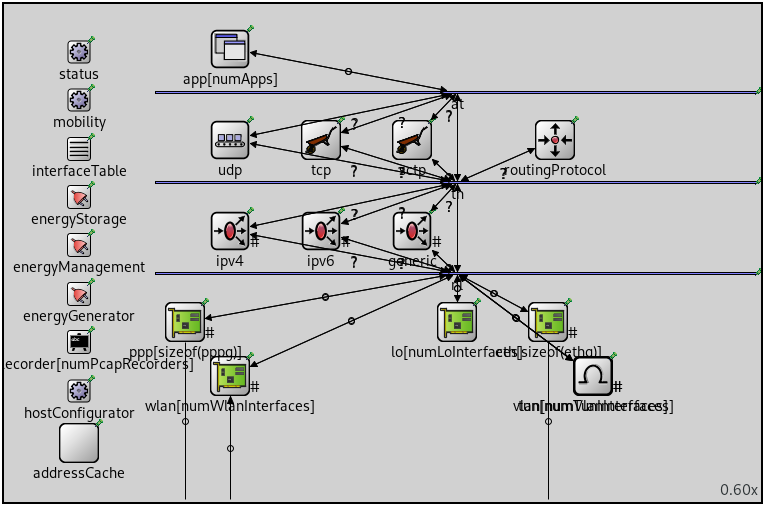
\includegraphics[width=1\textwidth]{static_host}
\decoRule
\caption[Estructura del módulo \code{StaticHost}]{Estructura del módulo
\code{StaticHost}.}
\label{fig:static_host}
\end{figure}

De manera similar, el módulo \code{Car} hereda del módulo \code{AdhocHost} de
INET, e incluye los módulos \code{CarMobility}, \code{CarConfigurator} y
\code{RoutingProtocolCar}. Su estructura se muestra en la figura \ref{fig:car}.

\begin{figure}[th!]
\centering
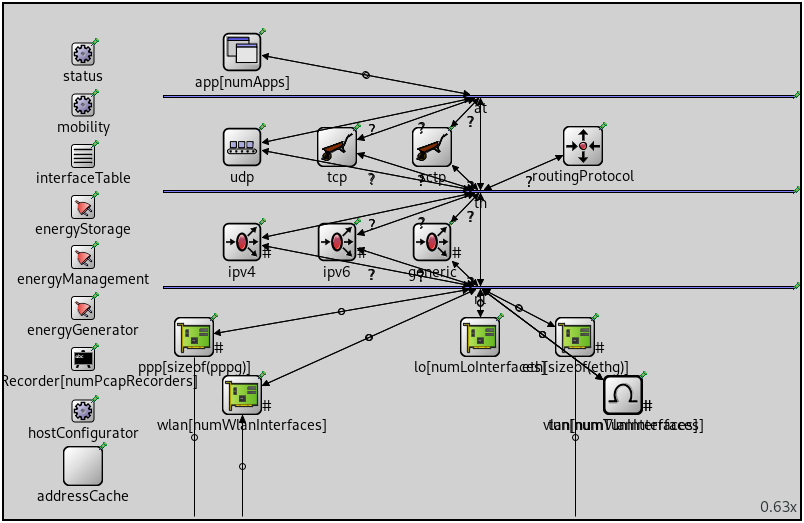
\includegraphics[width=1\textwidth]{car}
\decoRule
\caption[Estructura del módulo \code{Car}]{Estructura del módulo \code{Car}.}
\label{fig:car}
\end{figure}
